
\section{Feature set}

\subsection{Motivación}

\begin{frame}
\frametitle{¿Cómo transformar la posición a un vector?}
\begin{figure}
\centering
\includegraphics<1>[width=1.0\linewidth]{../assets/slides/fs_motiv.pdf}
\includegraphics<2>[width=1.0\linewidth]{../assets/slides/fs_motiv2.pdf}
\end{figure}
\end{frame}

\subsection{Definición}

\begin{frame}
\frametitle{Definición}
\begin{figure}
Un \textbf{feature set} $\bm{S_P}$ se define con un conjunto $\bm{S}$ y\\ un predicado asociado $\bm{P(e)}$, donde: \\
\vspace{0.5cm}
\begin{itemize}
    \item $\bm{S}$ es un conjunto de conceptos (rol, color, celda, número, etc.).
    \item $\bm{P(e)}$ es un predicado que determina si $e$ está presente (o \textit{activo}) en la posición (implícita).
    \vskip 0.6cm
    \item<2-> Cada elemento en $S_P$ es un \textit{feature}.
    \item<3-> Cada \textit{feature} es un valor en el vector de entrada, valiendo 1 si está \textit{activo} y 0 si no.
\end{itemize}
\end{figure}
\end{frame}


\begin{frame}
\frametitle{Ejemplos de $S$}
Información posicional:

\begin{center}
\begin{tabular}{cc}

$\begin{aligned}[t]
\featureset{Files} &= \{a, b, ..., h\} \\
\featureset{Ranks} &= \{1, 2, ..., 8\} \\
\featureset{Squares} &= \{a1, a2, ..., h8\}
\end{aligned}$

&

\raisebox{-10ex}{
\chessboard[
    clearboard,
    tinyboard,
    showmover=false,
    pgfstyle={text},
    %text=\fontsize{1.2ex}{1.2ex}\bfseries\sffamily \thepieceindex \stepcounter{pieceindex}, %  \currentwq
    text=\fontsize{1.2ex}{1.2ex}\bfseries\sffamily \currentwq,
    markboard
]
}

\end{tabular}
\end{center}

Información sobre las piezas:

\begin{center}
$\begin{aligned}[t]
\featureset{Roles} &= \text{\{
    \sympawn\ Pawn,
    \symknight\ Knight,
    \symbishop\ Bishop,
    \symrook\ Rook,
    \symqueen\ Queen,
    \symking\ King\}}\textsuperscript{1} \\
\featureset{Colors} &= \text{\{\white\ White, \black\ Black\}}
\end{aligned}$
\end{center}


\end{frame}


\begin{frame}
\frametitle{Ejemplo completo}
\begin{figure}
\centering
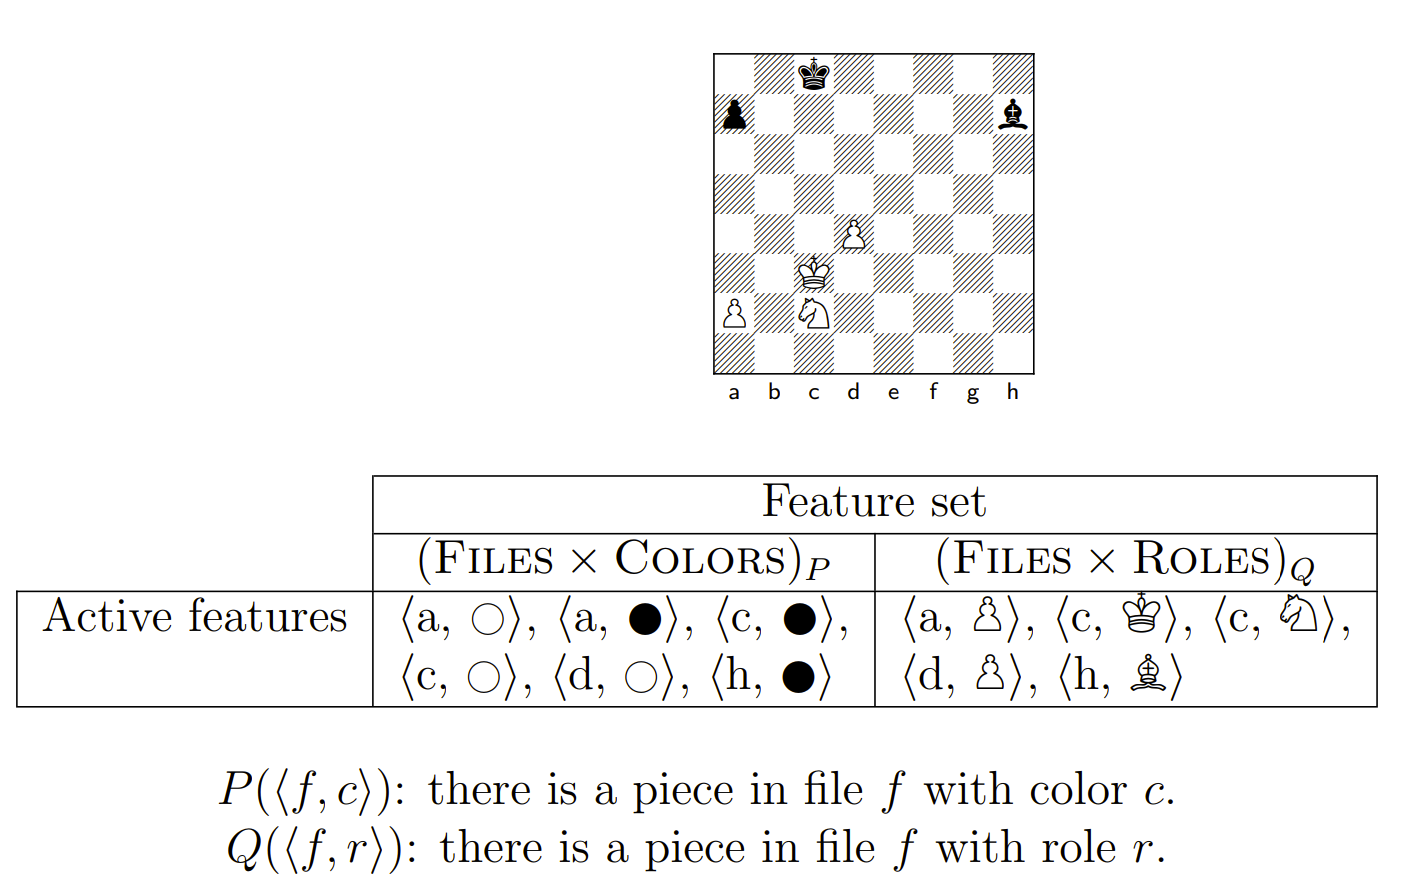
\includegraphics[width=1.0\linewidth]{../assets/slides/fs.png}
\end{figure}
\end{frame}